
\documentclass{article}
\usepackage{utf8math,ttquot,mathpartir,amsmath, amssymb, hydrocomments, mathtools,multicol,xspace}
\usepackage[margin=1in]{geometry}
\begin{document}

\section{syntax}

\newcommand{\closedprogram}{\textit{closed-program}\xspace}
\newcommand{\compiledcomponent}{\textit{compiled-component}\xspace}
\newcommand{\incast}{\textit{incast}\xspace}
\newcommand{\outcast}{\textit{outcast}\xspace}
\newcommand{\seqstart}{\textit{seq-start}\xspace}
\newcommand{\seqend}{\textit{seq-end}\xspace}
\newcommand{\chain}{\textit{chain}\xspace}
\newcommand{\op}{\textit{op}\xspace}
\newcommand{\opt}{τ_{\textit{op}}\xspace}
\newcommand{\N}{ℕ}
\newcommand{\fresh}{\textit{fresh}\xspace}

\begin{figure}
  \begin{align*}
    \closedprogram &:= "declare"~ A…~"in"~ \compiledcomponent…\\
    A &∈ \textit{handoff-names}\\
    \compiledcomponent &:= \incast;\outcast ∣ [\incast ∣ …]\op[\outcast ∣ …] \\
    \incast &= A; \chain ∣ [\incast ∣ …]\op;\chain\\
    \outcast &= \chain; A ∣ \chain; \op[\outcast ∣ …]\\
  \end{align*}
  \label{fig:syntax}
  \caption{Syntax}
\end{figure}


In figure \ref{fig:syntax}

\section{types}

\begin{figure}
    \begin{mathpar}
      \inferrule{C,A : d ⊢ "declare"~\textit{rest}…~"in"~\compiledcomponent}{C ⊢ "declare"~A, \textit{rest}…~"in"~\compiledcomponent}
      
      \inferrule{C ⊢ \incast \\ C ⊢ \outcast}{C ⊢ "declare"~"in"~\incast;\outcast}

      \inferrule{C ⊢ [\incast ∣ …]\op_{α} \\ C ⊢ \op_{α}[\outcast ∣ …] \\ α~\fresh \\\text{something for operator}}{C ⊢ "declare"~"in"~[\incast…]\op[\outcast…]}
      
    \end{mathpar}
    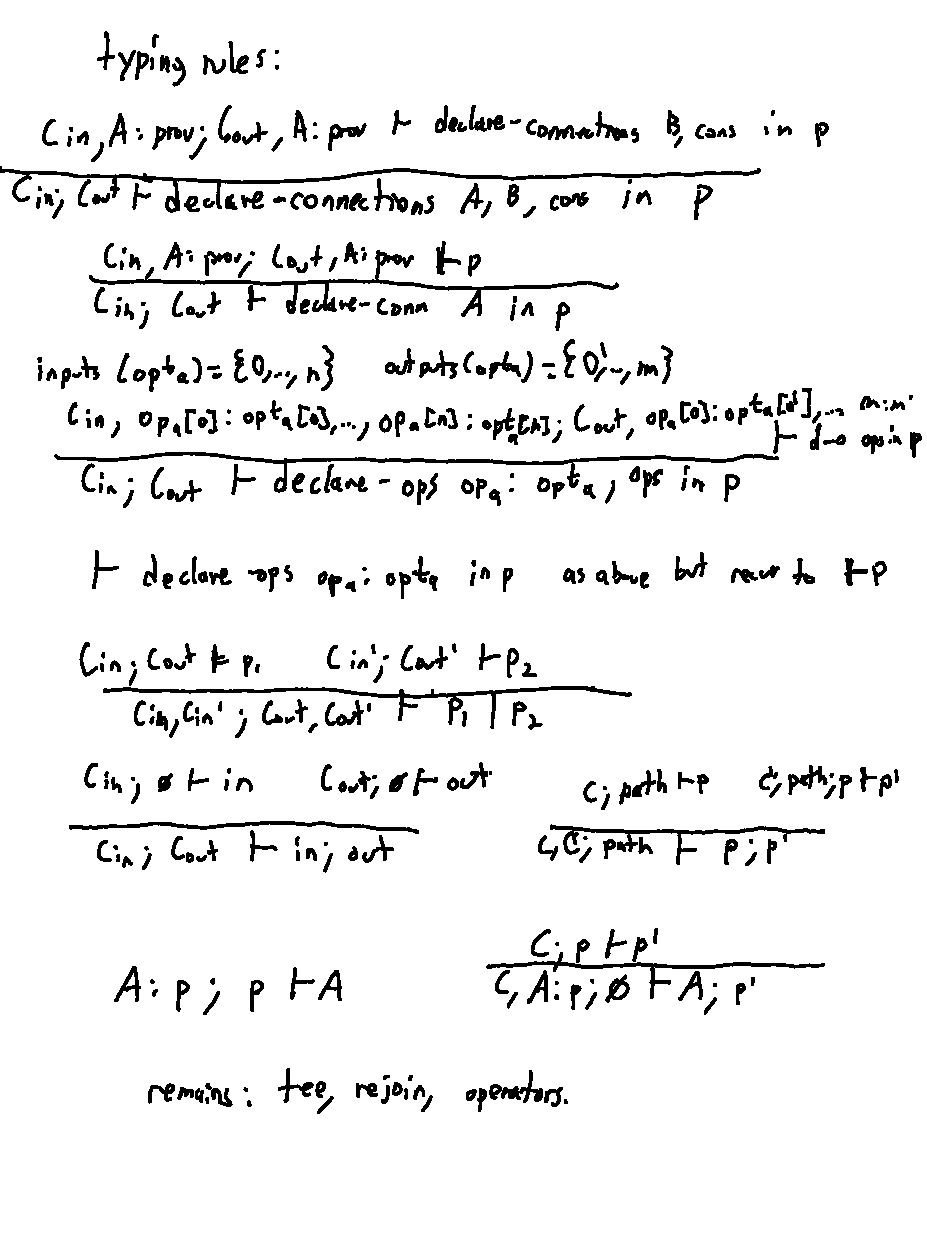
\includegraphics{freehand-types}
  \label{fig:types}
  \caption{Types}
\end{figure}

I feel like we need to put operators in the environment if we want to
be able to do the incast-outcast split. In fact, I feel like we might
have a derivation problem _in general_ when doing the incast-outcast
split. Annoying!


In figure \ref{fig:types}


\end{document}
